\documentclass[11pt]{article} % Font size (can be 10pt, 11pt or 12pt) and paper size (remove a4paper for US letter paper)

\usepackage{amsmath,amssymb,amsthm,gensymb}

\usepackage{geometry}
\usepackage{wrapfig}
\usepackage{hyperref}
\hypersetup{
    colorlinks=true,
    linkcolor=black,
    filecolor=magenta,      
    urlcolor=blue,
}
\usepackage[protrusion=true,expansion=true]{microtype} % Better typography
\usepackage{hyperref}
\usepackage{graphicx} % Required for including pictures
\usepackage{wrapfig} % Allows in-line images
\linespread{1.12}
\usepackage{mathtools}
\usepackage[font=footnotesize,labelfont=bf]{caption}
\usepackage[T1]{fontenc} % Required for accented characters

\makeatletter

\newcommand{\bra}[1]{\left\langle #1 \right|}
\newcommand{\ket}[1]{\left|#1\right\rangle}
\newcommand{\braket}[2]{\left\langle#1 |  #2\right\rangle}
\makeatother

%\addbibresource{bibliography.bib}


\author{Amir Karamlou\footnote{Notes LaTeXed by Megan Yamoah for 6.s089 IAP 2019.}\\\href{mailto:karamlou@mit.edu}{karamlou@mit.edu}}
\title{Introduction to Quantum Computing\\Lecture 2: Introduction to Quantum Mechanics II}
\date{Massachusetts Institute of Technology\\6.s089 IAP 2020}

\begin{document}
\maketitle
\newpage
\tableofcontents
\newpage


\section{Postulates of QM} \label{pos}
To gain a more technical and intuitive understanding of quantum mechanics, we discuss the postulates of the theory. There are six postulates which dictate the basis of quantum mechanical theory. We model our discussion around MIT Professor Jaffe's \href{http://web.mit.edu/8.05/handouts/jaffe1.pdf}{notes} from 8.05 as taught in 1996 (basic quantum mechanics has not really changed since then). This section will provide many of the important consequences involving quantum operators and measurement that are significant for quantum computing.

\subsection{First Postulate}
\begin{center}
    \textit{A quantum state is represented by a ket, some $\ket{\psi}$ in the state space, called a wavefunction. It completely specifies the quantum state.}
\end{center}

The space of states is a vector space which means that the superposition of two states is again a state of the system. This allows us to define arbitrary states $\ket{\psi} = \sum^\textrm{n}_ia_i\ket{e_i}$ for basis vectors $\ket{e_i}$ of the n-dimensional state space. This describes phenomena like the double-slit diffraction of electrons.

As a Hilbert space, the space of states has with it a defined inner product. Namely,
\begin{align}
    \left(\ket{\psi},\ket{\phi}\right) \equiv \braket{\psi}{\phi} = \int dx\psi^\ast(x)\phi(x)
\end{align}

We first define the inner product as an operation acting on two states in the ket space. Then the second step introduces the ``bra space" of the same dimension as the ket space, and defines the inner product as an operation involving one element of the each space. Finally, we reduce to the familiar continuous inner product which represents the overlap of $\ket{\psi}$ and $\ket{\phi}$. This notation allows us to see clearly that
\begin{align}
    \braket{\psi}{\phi}^\ast = \braket{\phi}{\psi}.
\end{align}

\subsection{Second Postulate}
\begin{center}
    \textit{Classical observables are introduced into quantum mechanics using operators. Specifically, every observable (measurable property) of a physical system is described by an operator that acts state kets.}
\end{center}

Classical observables (such as position $x$ or momentum $p$) are made ``quantum" by transforming them into quantum operators. One simply adds the operator hat ( $\hat{ }$ ) on top of the observable's variable.

Notation-wise, an operator acts on a state from the left, ie. $\textrm{\^A}\ket{\psi}$. In general, an operator acting on a state will change the state. For every operator, there are, however, states which are not changed by the action of the operator, giving, for example,
\begin{align}
\textbf{\^A}\ket{\psi_i} = a_i\ket{\psi_i}
\end{align}

\noindent These states are eigenstates to the operator and the value $a_i$ is the eigenvalue which represents the observable's value. An operator acting on a state which is not one of its eigenstates, will produce a probabilistic outcome based on the states representation in the basis of eigenstates for the operator. In this case, the operator will also change the quantum state of the system.

\subsection{Third Postulate} \label{third_pos}
\begin{center}
    \textit{The result of a measurement of an observable with an operator \textbf{\^A} will only ever be an eigenvalue of \textbf{\^A}.}
\end{center}

This postulates leads to the ``quantum" or ``quantized" nature of quantum mechanics. Some operators, like the position \textbf{\^x} or momentum \textbf{\^p} operators, have a set of continuous eigenvalues, so this proposition is not far removed from what we are used to from classical mechanics. However, for operators with discrete eigenvalues such as the Hamiltonian (ie. energy) operator for particle in a bound well, this proposition creates an unintutive result.

We note an important requirement here. First, measured values, in other words, the eigenvalues, must be real since these are real, classically measured observables. This means that operators corresponding to an observable must be Hermitian (remember Section \ref{operators}). Hermitian operators also have eigenstates which form a complete basis which means that any state in the space can be decomposed into a linear superposition of eigenstates of the operator. These operators can be re-written as $\textbf{\^A} = \sum_i\lambda_i\ket{a_i}\bra{a_i}$ for eigenvalues $\lambda_i$ and corresponding eigenvectors $\ket{a_i}$.

\subsection{Fourth Postulate} \label{fourth_pos}
\begin{center}
    \textit{When a measurement of an observable with operator \textbf{\^A} is made on a generic state $\ket{\psi}$, the probability of obtaining a certain eigenvalue $a_i$ is given by the square of the inner product of $\ket{\psi}$ with the corresponding eigenstate $\left|\braket{a_i}{\psi}\right|^2$.}
\end{center}

Professor Jaffe gives a very good treatment of this postulate, so we abbreviate them here.

We assume that the states are normalized which is in general possible. States are usually normalized to unity,
\begin{align}
    \braket{\psi}{\psi} &= 1\nonumber\\
    \braket{a_j}{a_k} &= \delta_{jk}
\end{align}

The complex number, $\braket{a_i}{\psi}$ is known as the ``probability amplitude", to measure $a_i$ as the value for the observable \textbf{A} in the state $\ket{\psi}$.

The postulate suggests the following algebraic exercise. First, any state can be expanded as a superposition of \textbf{\^A}-eigenstates (see Postulate 3),
\begin{align}
    \ket{\psi} = \sum_nc_n\ket{a_n}.
\end{align}

Next use the orthonormality of the \textbf{\^A}-eigenstates to find an expression for the expansion coefficients $c_n$,
\begin{align}
    \braket{a_j}{\psi} &= \sum_nc_n\braket{a_j}{a_n}\\
    &= c_j.
\end{align}

So,
\begin{align}
    \ket{\psi} = \sum_n\braket{a_n}{\psi}\ket{a_n}
\end{align}

where we have the complex number $\braket{a_n}{\psi}$ and the state $\ket{a_n}$. The component of $\ket{\psi}$ along the direction of the nth eigenstate of \textbf{\^A} is given by $\braket{a_n}{\psi}$. The measurement operation yields the result $a_n$ with a probability proportional to the square of this component, $\left|\braket{a_n}{\psi}\right|^2$.

The probability of obtaining some result at all is unity. For states normalized to unity,
\begin{align}
    \left|\braket{\psi}{\psi}\right|^2 = \left|\sum_m\sum_nc_m^\ast c_n\braket{a_m}{a_n}\right|^2.
\end{align}

Using $\left|\braket{\psi}{\psi}\right|^2 = 1$ and $\braket{a_m}{a_n} = \delta_{mn}$, we get
\begin{align}
    \sum_n\left|c_n\right|^2 = 1.
\end{align}

According to the usual rules of probability, we can compute the ``expectation value" of the observable \textbf{A}. If the probability to observe $a_n$ is $\left|c_n\right|^2$, then the expected value
(denoted $\left<\textbf{A}\right>$) is
\begin{align}
    \left<\textbf{A}\right> = a_n\left|c_n\right|^2
\end{align}
as long as each eigenstate has a unique eigenvalue (the operator \textbf{\^A} has no degenerate eigenvalues).

\subsection{Fifth Postulate}
\begin{center}
    \textit{Immediately after the measurement of an observable \textbf{A} with a value $a_n$, the state of the system is the normalized eigenstate $\ket{a_n}$.}
\end{center}

This postulate gives way to the idea of the ``collapse of the wavepacket". While measuring a state $\ket{\psi}$ for the observable \textbf{A} gives the value $a_n$ with probability $\left|\braket{a_n}{\psi}\right|$, results for remeasuring immediately after the first measurement are not statistically distributed. Namely, after measurement, the state $\ket{\psi}$ is found in the renormalized state $\ket{a_n}$ since the outcome is always $a_n$.

Wavefunction collapse is one of the more unintuitive concepts in quantum mechanics, but is supported by experimental results with repeated measurements.

\subsection{Sixth Postulate}
\begin{center}
    \textit{Quantum states generally change (evolve) with time. This time evolution preserves the normalization of the state. The time evolution of the state of a quantum system is described by $\ket{\psi(t)} = \textbf{\^U}(t,t_0)\ket{\psi(t_0)}$, for some unitary operator \^U.}
\end{center}

A quantum state must evolve by a unitary operator since the norm of the state must be preserved. While individual probabilities of a observing certain eigenvalues of an operator may change, the total sum ($\sum_n\left|c_n\right|^2$ from before) remains the same. The probability for measuring some value of any operator remains unity.

As such, for a state evolving with time $\ket{\psi(t)}$, we maintain $\left|\braket{\psi(t)}{\psi(t)}\right|^2 = 1$ for all $t$. So,
\begin{align}
    \left|\braket{\psi(t)}{\psi(t)}\right|^2 &= 1\\
    &= \left|\bra{\psi(t_0)}\textbf{\^U}^\dagger(t,t_0)\textbf{\^U}(t,t_0)\ket{\psi(t_0)}\right|^2\nonumber\\
    &= \left|\braket{\psi(t_0)}{\psi(t_0)}\right|^2 = 1,
\end{align}
which is consistent with our earlier requirement for a unitary operator. This also means that time evolution is a reversible process. We reverse some time evolution given by $\textbf{\^U}(t,t_0)$ we simply act with $\textbf{\^U}(t_0,t) = \textbf{\^U}^\dagger(t,t_0)$.

This postulate actually leads to the Schr\"odinger equation which requres that a state $\ket{\psi}$ evolves under
\begin{align}
    i\hbar\frac{d}{dt}\ket{\psi(t)} = \mathcal{H}\ket{\psi(t)}
\end{align}
for a Hermition operator $\mathcal{H}$ which is a system-dependent operator called the Hamiltonian.

\section{Uncertainty Principle}

The postulates of quantum mechanics highlight the probabilistic nature of the theory. This in turn gives rise to some interesting (and sometime unintuitive or even concerning) phenomena. One of these is the uncertainty principle which states that there is a limit to the precision with which one is able to determine the values of conjugate observables (such as position and momentum and energy and time).

Stepping back to classical probability theory, we can define an expectation value $\left<\textbf{A}\right>$, variance $(\Delta\textbf{A})^2$, and standard deviation $(\Delta\textbf{A})$ such that for possible values $a_i$ each with probability $p_i$,
\begin{align}
    \left<\textbf{A}\right> &= \sum_ia_ip_i,\\
    (\Delta\textbf{A})^2 &= \left<\left(\textbf{A}-\left<\textbf{A}\right>\right)^2\right> = \left<\textbf{A}^2\right> - \left<\textbf{A}\right>^2,\\
\end{align}
and
\begin{align}
    \Delta\textbf{A} = \sqrt{\left<\textbf{A}^2\right> - \left<\textbf{A}\right>^2}.
\end{align}

Using the fourth postulate, we can then apply this to quantum mechanics and relate the product of the standard deviations of two operators to their commutator. More explicitly, we use $p_i = \left|\braket{\psi}{\phi_i}\right|^2$ to find $\Delta\textbf{A}\Delta\textbf{B}$ in terms of $[\textbf{A},\textbf{B}]$. The standard deviation $\Delta\textbf{A}$ measures the uncertainty in our knowledge of the value of the observable \textbf{A}, so we will be placing a limit on our this uncertainty.

First, in quantum mechanics, the expectation value of an observable simplifies to
\begin{align}
    \left<\textbf{A}\right> &= \sum_ia_ip_i\nonumber\\
    &= \sum_ia_i\braket{\psi}{\phi_i}\braket{\phi_i}{\psi}\\
    &= \bra{\psi}\left(\sum_ia_i\ket{\phi_i}\bra{\phi_i}\right)\ket{\psi}\nonumber\\
    &= \bra{\psi}\textbf{A}\ket{\psi}.
\end{align}

To derive the uncertainty principle, let
\begin{align}
    \bra{\psi}\textbf{AB}\ket{\psi} = re^{i\phi}
\end{align}
where $re^{i\phi}$ represents some arbitrary complex number. Using $\bra{\psi}\textbf{AB}\ket{\psi}^\dagger = \bra{\psi}\textbf{BA}\ket{\psi}$ for Hermitian operators \textbf{\^A} and \textbf{\^B}, one finds
\begin{align}
    \bra{\psi}\textbf{AB}-\textbf{BA}\ket{\psi} = re^{i\phi} - re^{-i\phi} = 2ir\sin\phi,\\
    \bra{\psi}\textbf{AB}+\textbf{BA}\ket{\psi} = re^{i\phi} + re^{-i\phi} = 2r\cos\phi,
\end{align}{}
and
\begin{align}
    \left|\bra{\psi}\textbf{AB}+\textbf{BA}\ket{\psi}\right|^2 + \left|\bra{\psi}\textbf{AB}-\textbf{BA}\ket{\psi}\right|^2 = 4r^2.
    \label{uncertainty_mag}
\end{align}
Thus follows
\begin{align}
    \left|\bra{\psi}\textbf{AB}-\textbf{BA}\ket{\psi}\right|^2 \leq 4\left|\bra{\psi}\textbf{AB}\ket{\psi}\right|^2
\end{align}
since both arguments on the left side of 
Eq. \ref{uncertainty_mag} are necessarily greater than or equal to zero. One further reduces using the inner product inequality from linear algebra to find
\begin{align}
    \frac{\left|\bra{\psi}\left[\textbf{A},\textbf{B}\right]\ket{\psi}\right|^2}{4} \leq \bra{\psi}\textbf{A}^2\ket{\psi}\bra{\psi}\textbf{B}^2\ket{\psi}.
\end{align}

Now, define $\textbf{A} = \textbf{C} - \left<\textbf{C}\right>$ and $\textbf{B} = \textbf{D} - \left<\textbf{D}\right>$ where $\left[\textbf{A},\textbf{B}\right] = \left[\textbf{C},\textbf{D}\right]$, $\bra{\psi}\textbf{A}^2\ket{\psi} = \left(\Delta\textbf{C}\right)^2$, and $\bra{\psi}\textbf{B}^2\ket{\psi} = \left(\Delta\textbf{D}\right)^2$. So,
\begin{align}
    \left|\frac{\bra{\psi}\left[\textbf{C},\textbf{D}\right]\ket{\psi}}{2}\right|^2 \leq \left(\Delta\textbf{C}\right)^2\left(\Delta\textbf{D}\right)^2,
\end{align}
which brings us to the Heisenberg Uncertainty principle:
\begin{align}
    \frac{\bra{\psi}\left[\textbf{C},\textbf{D}\right]\ket{\psi}}{2} \leq \Delta\textbf{C}\Delta\textbf{D}.
\end{align}

This statement gains significance when we considering the position and momentum conjugate variables. Since $\left[\textbf{\^x},\textbf{\^p}\right] = i\hbar$, $\Delta\textbf{\^x}\Delta\textbf{\^p} \geq \frac{\hbar}{2}$, so one can only measure together the position and momentum variables of a system to a minimum of $\frac{\hbar}{2}$. Increasing knowledge about the position of a system necessarily decreases the knowledge an observer can have about the momentum of a system (and vice versa). This is true for all non-communiting observables.

\section{Local Hidden Variables}

Einstein was rather uncomfortable with the idea that quantum mechanics was a fundamentally probabilistic theory\footnote{as shown by his famous statement ``God does not play dice.''}. He say quantum mechanics as akin to thermodynamics which describes macroscopic effects using derivations from microscopic or ``hidden'' variables. We illustrate this idea with an example using a system of three (two-state) quantum spins (like an atom or a qubit, for example). This system has a total Hilbert space
\begin{align}
\mathcal{H} = \mathcal{H}^{\otimes3}_\textrm{spin} = \mathcal{H}^A_\textrm{spin}\otimes\mathcal{H}^B_\textrm{spin}\otimes\mathcal{H}^C_\textrm{spin}.
\end{align}

For a given state $\ket{\psi}$, one cannot predict the outcome of measuring each spin along a single axis. However, one could assume that each spin has a secret (secret to the observer) setting: either $\uparrow = +1$ or $\downarrow = -1$ for each of $x$, $y$, and $z$ for each spin. We label these $S^1_x$ for an $\textbf{\^x}$ measurement on the first qubit, and so on. As such, the system has its own truth table, so to speak, which determines the outcome of any measurement on the system (say, $\textbf{\^x}_1\textbf{\^y}_2\textbf{\^y}_3$ or $\textbf{\^z}_1\textbf{\^x}_2\textbf{\^y}_3$).

In 1993, physicists Greenberger, Horne, and Zeilinger attempted to show the invalidity of local hidden variables. They wrote down a state, known as the GHZ state:
\begin{align}
    \ket{\Psi}_{GHZ} = \frac{1}{\sqrt{2}}\left(\ket{000} - \ket{111}\right)
\end{align}
for a system of three spins. We will measure the following operators on the GHZ state: $\textbf{\^x}_1\textbf{\^x}_2\textbf{\^x}_3$, $\textbf{\^x}_1\textbf{\^y}_2\textbf{\^y}_3$, $\textbf{\^y}_1\textbf{\^x}_2\textbf{\^y}_3$, $\textbf{\^y}_1\textbf{\^y}_2\textbf{\^x}_3$.

The expectation value of the first observable $x_1x_2x_3$ on the GHZ state is
\begin{align}
    \left<\textbf{\^x}_1\textbf{\^x}_2\textbf{\^x}_3\right>_{GHZ} &= \bra{\Psi}_{GHZ}\sigma^1_x\sigma^2_x\sigma^3_x\ket{\Psi}_{GHZ}\\
    &= \frac{1}{\sqrt{2}}\bra{\Psi}_{GHZ}\sigma^1_x\sigma^2_x\sigma^3_x\left(\ket{000} - \ket{111}\right)\nonumber\\
    &= \frac{1}{\sqrt{2}}\bra{\Psi}_{GHZ}\left(\ket{111} - \ket{000}\right)\nonumber\\
    &= -\frac{1}{\sqrt{2}}\bra{\Psi}_{GHZ}\left(\ket{000} - \ket{111}\right)\nonumber\\
    &= -\braket{\Psi}{\Psi}_{GHZ}\nonumber\\
    &= -1.
\end{align}
For $x_1y_2y_3$, the expectation value is
\begin{align}
    \left<\textbf{\^x}\textbf{\^y}\textbf{\^y}\right>_{GHZ} &= \frac{1}{\sqrt{2}}\bra{\Psi}_{GHZ}\sigma^1_x\sigma^2_y\sigma^3_y\left(\ket{000} - \ket{111}\right)\nonumber\\
    &= \frac{1}{\sqrt{2}}\bra{\Psi}_{GHZ}\left(\ket{1}_A\left(i\ket{1}_B\right)\left(i\ket{1}_C\right) - \ket{0}_A\left(-i\ket{0}_B\right)\left(-i\ket{0}_C\right)\right)\nonumber\\
    &= -\frac{1}{\sqrt{2}}\bra{\Psi}_{GHZ}\left(-\ket{111} + \ket{000}\right)\nonumber\\
    &= \braket{\Psi}{\Psi}_{GHZ}\nonumber\\
    &= 1
\end{align}
as is the expectation values for $y_1x_2y_3$ and $y_1y_2x_3$.

We have, then
\begin{align}
    \left<\textbf{\^x}\textbf{\^x}\textbf{\^x}\right>\left<\textbf{\^x}\textbf{\^y}\textbf{\^y}\right>\left<\textbf{\^y}\textbf{\^x}\textbf{\^y}\right>\left<\textbf{\^y}\textbf{\^y}\textbf{\^x}\right> &= (-1)(+1)(+1)(+1)\nonumber\\
    &= -1.
\end{align}
However, if we calculate this same value using the hidden variables approach, we find
\begin{align}
    \left(S^1_xS^2_xS^3_x\right)\left(S^1_xS^2_yS^3_y\right)\left(S^1_yS^2_xS^3_y\right)\left(S^1_yS^2_yS^3_x\right) &= \left(S^1_x\right)^2\left(S^1_y\right)^2\left(S^2_x\right)^2\left(S^2_y\right)^2\left(S^3_x\right)^2\left(S^3_y\right)^2\nonumber\\
    &= (\pm1)^2\nonumber\\
    &= +1,
\end{align}
which is clearly a contradiction. So, if quantum mechanics is correct, as research and experiment suggest, our world really is probabilistic after all\footnote{Sorry, Mr. Einstein.}.

\section{The Bloch Sphere}\label{block_sphere}
The Bloch sphere is a useful tool for visualizing qubit states (or any quantum state in $\mathcal{H}^2$. A pure quantum state is represented by a vector on the surface of a unit sphere (Fig \ref{fig:bloch}). The state $\ket{0}$ exists at the top of the sphere (the north pole) and the state $\ket{1}$ exists at the bottom (the south pole). Using spherical coordinates, arbitrary qubit states are defined on the sphere with $\ket{\psi} = \cos\frac{\theta}{2}\ket{0} + e^{i\phi}\sin\frac{\theta}{2}\ket{1}$ with polar angle $\theta$ and azimuthal angle $\phi$. Any state can be written $\ket{\psi} = e^{i\gamma}\left(\cos\frac{\theta}{2}\ket{0} + e^{i\phi}\sin\frac{\theta}{2}\ket{1}\right)$ where we factor out the phase associated with the $\ket{0}$ basis state. However, in quantum mechanics, the arbitrary phase $e^{i\gamma}$ has no observable effects on the state. So, any qubit state is described by a point on the unit sphere.
\begin{figure}[Bloch Sphere]
  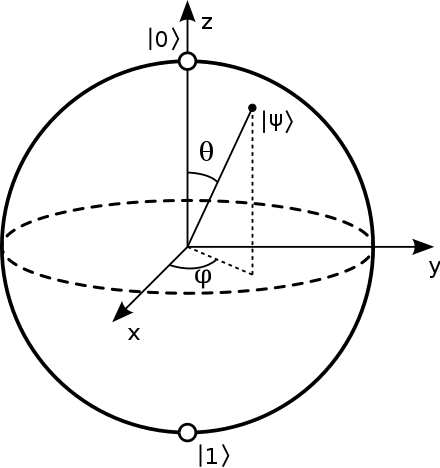
\includegraphics[scale=0.35]{Lecture3Figs/BlochSphere_diag.png}
  \caption{Bloch Sphere}
  \label{fig:bloch}
\end{figure}

Using this formula, we can define the states which match the positive and negative x, y, and z-axes as
\begin{align}
    +z &= \ket{0}\nonumber\\
    -z &= \ket{1}\nonumber\\
    +x &= \ket{+} = \frac{1}{\sqrt{2}}\left(\ket{0} + \ket{1}\right)\nonumber\\
    -x &= \ket{-} = \frac{1}{\sqrt{2}}\left(\ket{0} - \ket{1}\right)\nonumber\\
    +y &= \ket{+i} = \frac{1}{\sqrt{2}}\left(\ket{0} + i\ket{1}\right)\nonumber\\
    -y &= \ket{-i} = \frac{1}{\sqrt{2}}\left(\ket{0} - i\ket{1}\right)
\end{align}
which one can prove to oneself using appropriate values for $\theta$ and $\phi$.

Let's consider the action of the Pauli matrices on states on the Bloch sphere. We will find that they, when exponentiated, generate rotations. Specifically, a rotation along some axis \^n is represented by
\begin{align}
    R_n(\theta) &= e^{-i\frac{\theta}{2}\textrm{\^n}\cdot\vec{\sigma}}\\
    &= \cos\frac{\theta}{2} I - i\sin\frac{\theta}{2} \textrm{\^n}\cdot\vec{\sigma}
\end{align}
where $\vec{\sigma}$ is the ``vector" of Pauli matrices. In the second line, we use the fact that $\sigma_i^2 = 1$ for the Paulis. In the following, we show that the above truly is a rotation on the Bloch sphere.

To do so, it is useful to consider the density operator formed by the outer product of the qubit state:
\begin{align}
    \rho &= \ket{\psi}\bra{\psi} = \ket{\psi}\otimes\bra{\psi}\\
    &=
        \begin{pmatrix}
            \cos^2\frac{\theta}{2} & e^{-i\phi}\cos\frac{\theta}{2}\sin\frac{\theta}{2} \\
            e^{i\phi}\cos\frac{\theta}{2}\sin\frac{\theta}{2} & \sin^2\frac{\theta}{2}
        \end{pmatrix}\nonumber\\
    &= \frac{1}{2}
        \begin{pmatrix}
            1+\cos\theta & \cos\phi\sin\theta - i\sin\phi\sin\theta \\
            \cos\phi\sin\theta + i\sin\phi\sin\theta & 1-\cos\theta
        \end{pmatrix}\\
    &= \frac{1}{2}\left(I+X\cos\phi\sin\theta + Y\sin\phi\sin\theta+Z\cos\theta\right)\\
    &= \frac{1}{2}\left(I+\vec{r}_\rho\cdot\vec{\sigma}\right)
\end{align}
where we have $I, X, Y, Z$ as the identity and Pauli matrices and $\vec{r}_\rho = (r_x,\;r_y,\;r_z) = (\cos\phi\sin\theta,\;\sin\phi\sin\theta,\;\cos\theta)$ as a unit vector in spherical coordinates.

The action of an operator on a quantum state must obey unitary evolution, preserving the norm of the state. The action of a unitary operator on a state can we used to find the action on the density operator $\rho$. Since a unitary operator $\hat{U}$ acting on a state $\ket{\psi}$ is given by $\ket{\psi} \rightarrow \textrm{\^U}\ket{\psi}$, the action of the operator on $\rho$ is
\begin{align}
    \rho = \ket{\psi}\bra{\psi} \rightarrow \textrm{\^U}\ket{\psi}\bra{\psi}\textrm{\^U}^\dagger.
\end{align}

Our rotation matrix is unitary since the Pauli matrices are Hermitian. Let's observe the action of a z-axis rotation on our density matrix. For a rotation around the z-axis, $R_z(\theta) = cos\frac{\theta}{2}I-i\sin\frac{\theta}{2}\sigma_z$. Since $\rho$ is a sum of the Pauli matrices, we can evaluate $R_z(\theta)$ on each individually:
\begin{align}
    \rho' &= R_z(\theta)\rho R_z(\theta)^\dagger\\
    &= \frac{1}{2}\left(I+r_x R_z(\theta)X R_z(\theta)^\dagger +r_y R_z(\theta)Y R_z(\theta)^\dagger + r_z R_z(\theta)Z R_z(\theta)^\dagger\right).
\end{align}
For the first term, the we use the unitary property of the rotation matrix.

Expanding the $X$ term, we have
\begin{align}
    R_z(\theta)X R_z(\theta)^\dagger &= \left(\cos\frac{\theta}{2}I-i\sin\frac{\theta}{2}\sigma_z\right)X\left(\cos\frac{\theta}{2}I+i\sin\frac{\theta}{2}\sigma_z\right)\\
    &= \cos^2\frac{\theta}{2}X + i\sin\frac{\theta}{2}\cos\frac{\theta}{2}XZ - i\sin\frac{\theta}{2}\cos\frac{\theta}{2}ZX+\sin^2\frac{\theta}{2}ZXZ\\
    &= \cos^2\frac{\theta}{2}X + \sin\frac{\theta}{2}\cos\frac{\theta}{2}Y + \sin\frac{\theta}{2}\cos\frac{\theta}{2}Y - \sin^2\frac{\theta}{2}X\\
    &= \left(\cos^2\frac{\theta}{2}-- \sin^2\frac{\theta}{2}\right)X + 2\sin\frac{\theta}{2}\cos\frac{\theta}{2}Y\nonumber\\
    &= \cos\theta X + \sin\theta Y.
\end{align}
Similarly, we can show\footnote{Give it shot!}
\begin{align}
    R_z(\theta)Y R_z(\theta)^\dagger &= \cos\theta Y - \sin\theta X\\
    R_z(\theta)Z R_z(\theta)^\dagger &= Z.
\end{align}
Now, rewriting $\rho'$,
\begin{align}
    \rho' &= \frac{1}{2}\left(I+r_x R_z(\theta)X R_z(\theta)^\dagger +r_y R_z(\theta)Y R_z(\theta)^\dagger + r_z R_z(\theta)Z R_z(\theta)^\dagger\right)\nonumber\\
    &= \frac{1}{2}\left(I+r_x \cos\theta X + \sin\theta Y +r_y \cos\theta Y - \sin\theta X + r_z Z\right)\nonumber\\
    &= \frac{1}{2}\left(I+(r_x\cos\theta-r_y\sin\theta)X + (r_x\sin\theta+r_y\cos\theta)Y + r_z Z\right)\\
    &= \frac{1}{2}\left(I+r_x'X + r_y'Y+r_z'Z\right)
\end{align}
where we have the transformed positions
\begin{align}
    r_x' &= r_x\cos\theta-r_y\sin\theta\nonumber\\
    r_y' &= r_x\sin\theta+r_y\cos\theta\nonumber\\
    r_z' &= r_z
\end{align}
which match exactly what we expect from a rotation around the z-axis. We can then construct the $R_z(\theta)$ rotation matrix
\begin{align}
    \begin{pmatrix}
        \cos\theta & -\sin\theta & 0\\
        \sin\theta & \cos\theta & 0\\
        0 & 0 & 1
    \end{pmatrix}.
\end{align}
We can do something similar to construct the matrix for a rotation around an arbitrary axis by making composite rotations with $R_x$, $R_y$, and $R_z$.

\subsection{Density Matrix}
The density matrix is a powerful construct that allows us to, for example, compare quantum states with classical statistics and consider the effect of measurements. We define the density matrix $\rho$:
\begin{align}
    \rho = \ket{\psi}\bra{\psi}
\end{align}
as in Section \ref{block_sphere}.

As an example, we can use the density matrix to determine the difference between a coin flip and an equal quantum superposition.

We term processes that take the off-diagonal elements to zero ``decoherence", which is an important negative effect which is, for many architectures, the main obstacle toward scalable quantum processors.


\end{document}